\documentclass[conference]{IEEEtran}

% Fix for UTF-8 encoding issues
\usepackage[utf8]{inputenc}

% Additional packages
\usepackage{graphicx}
\usepackage{amsmath}
\usepackage{url}
\usepackage{fancyhdr}
\usepackage{color}
\usepackage{hyperref}
\usepackage{subcaption}

\definecolor{headergray}{gray}{0.6}
\addtolength{\topmargin}{10pt}

% Title and author block
\title{Titanic Survival Prediction: Pure ID3 Algorithm Implementation}
\author{
\IEEEauthorblockN{Francesco Albano}
\IEEEauthorblockA{
Student ID: LJ2506219\\
School of Computer Science\\
Beihang University (BUAA)\\
Beijing, China\\
Email: francescoalbano@buaa.edu.cn, francescoalbano357@gmail.com}
}
\begin{document}

\pagestyle{fancy}
\fancyhead[C]{\textcolor{headergray}{Assignment report for Artificial Intelligence}}
\renewcommand{\headrulewidth}{0pt}
\fancyfoot[C]{\thepage}
\setlength{\footskip}{40pt}

\maketitle

\begin{abstract}
This report presents a modular implementation of the pure ID3 decision tree algorithm for Titanic survival prediction. The project demonstrates theoretical understanding, advanced data preprocessing, and professional visualization, achieving 89.23\% accuracy on the training set. Depth optimization and feature engineering are discussed, with results and code structure provided for reproducibility.
\end{abstract}

\begin{IEEEkeywords}
ID3, decision tree, Titanic, machine learning, data preprocessing, interpretability
\end{IEEEkeywords}

\section{Introduction}
This project implements a Titanic passenger survival prediction system using the pure ID3 decision tree algorithm, following Professor Bai Xiao's specifications. The goal is to combine theoretical rigor with practical data science skills, focusing on modularity, accuracy, and visualization. The ID3 algorithm is chosen for its interpretability and educational value, allowing a transparent view of how decisions are made based on data features. The modular approach ensures that each phase of the workflow (preprocessing, learning, visualization) can be understood, tested e migliorato separatamente.

\section{System Architecture}
The project uses a modular design with four main components, each with a clear responsibility:
\begin{itemize}
    \item \textbf{id3\_core\_algorithm.py}: Implements the ID3 algorithm from scratch, including manual entropy and information gain calculations. This ensures full control and understanding of the learning process, without relying on external machine learning libraries.
    \item \textbf{data\_preprocessor.py}: Handles advanced data cleaning, optimal binning, and feature engineering. Preprocessing is crucial for improving model accuracy and robustness, especially with real-world datasets like Titanic, which contain missing values and outliers.
    \item \textbf{visualization\_export.py}: Generates charts, tree diagrams, and exports results to CSV. Visualization helps interpret the decision process and communicate results effectively.
    \item \textbf{main\_titanic\_id3.py}: Coordinates the workflow, integrating all modules and managing the analysis pipeline.
\end{itemize}

\section{Algorithm Implementation}
\subsection{ID3 Core Algorithm}
The \texttt{PureID3Algorithm} class implements the standard ID3 algorithm with manual entropy calculation:
\begin{equation}
E(S) = -\sum_{i=1}^{c} p_i \log_2(p_i)
\end{equation}
\begin{equation}
IG(S,A) = E(S) - \sum_{v \in Values(A)} \frac{|S_v|}{|S|} E(S_v)
\end{equation}
The implementation is recursive, building the tree by selecting at each node the feature with the highest information gain. Depth limiting is included to prevent overfitting and to allow analysis of the trade-off between accuracy and interpretability. All logic is written in pure Python, making the code accessible and modifiable for educational purposes. This approach allows to follow every step of the algorithm and understand the impact of each design choice.

\subsection{Data Preprocessing}
Advanced preprocessing techniques are applied to maximize the quality of the input data:
\begin{itemize}
    \item \textbf{Outlier handling}: Instead of removing outliers, values are capped using the interquartile range (IQR), preserving as much information as possible.
    \item \textbf{Optimal binning}: Continuous variables (Age, Fare) are discretized into bins chosen to maximize information gain, improving the algorithm's ability to split data meaningfully.
    \item \textbf{Feature engineering}: New features such as passenger title and family size are extracted, providing additional predictive power and interpretability.
    \item \textbf{Missing values}: Missing data is imputed using statistical methods (mode for categorical, median for numerical), reducing bias and maintaining dataset integrity.
\end{itemize}
These steps are essential for real-world datasets, where raw data is often noisy and incomplete. Good preprocessing directly impacts the performance and reliability of the final model.

\section{Results and Performance}
\subsection{Model Performance}
\begin{table}[h]
\centering
\begin{tabular}{|l|c|}
\hline
Metric & Value \\
\hline
Training Accuracy & 89.23\% \\
Total Samples & 891 \\
Correct Predictions & 795 \\
Tree Depth & 5 layers \\
Decision Rules & 207 \\
Total Nodes & 323 \\
\hline
\end{tabular}
\caption{Model Performance Summary}
\end{table}

\subsection{Depth Optimization Analysis}
\begin{table}[h]
\centering
\begin{tabular}{|c|c|c|c|}
\hline
Max Depth & Accuracy & Nodes & Evaluation \\
\hline
3 & 88.11\% & 295 & Good baseline \\
4 & 88.67\% & 309 & Gradual improvement \\
\textbf{5} & \textbf{89.23\%} & \textbf{323} & \textbf{Optimal balance} \\
6 & 89.90\% & 337 & Diminishing returns \\
Unlimited & 89.90\% & 450 & Overfitting risk \\
\hline
\end{tabular}
\caption{Depth Optimization Results}
\end{table}
Depth 5 was chosen for optimal balance between accuracy and interpretability.

\section{Visualization and Output}
High-quality decision tree diagrams are generated using scikit-learn's \texttt{plot\_tree} function, with color-coded nodes and readable labels. The generated tree (see Figure~\ref{fig:decisiontree}) makes the decision process transparent and easy to present in academic or professional contexts, evidenziando le regole e i criteri di suddivisione appresi dal modello. CSV exports include prediction results, feature importance, decision paths, and performance statistics, allowing further analysis and reproducibility. The visualization and export system is designed to support both learning and communication, making the results accessible to non-experts as well.

\begin{figure*}[t]
    \centering
    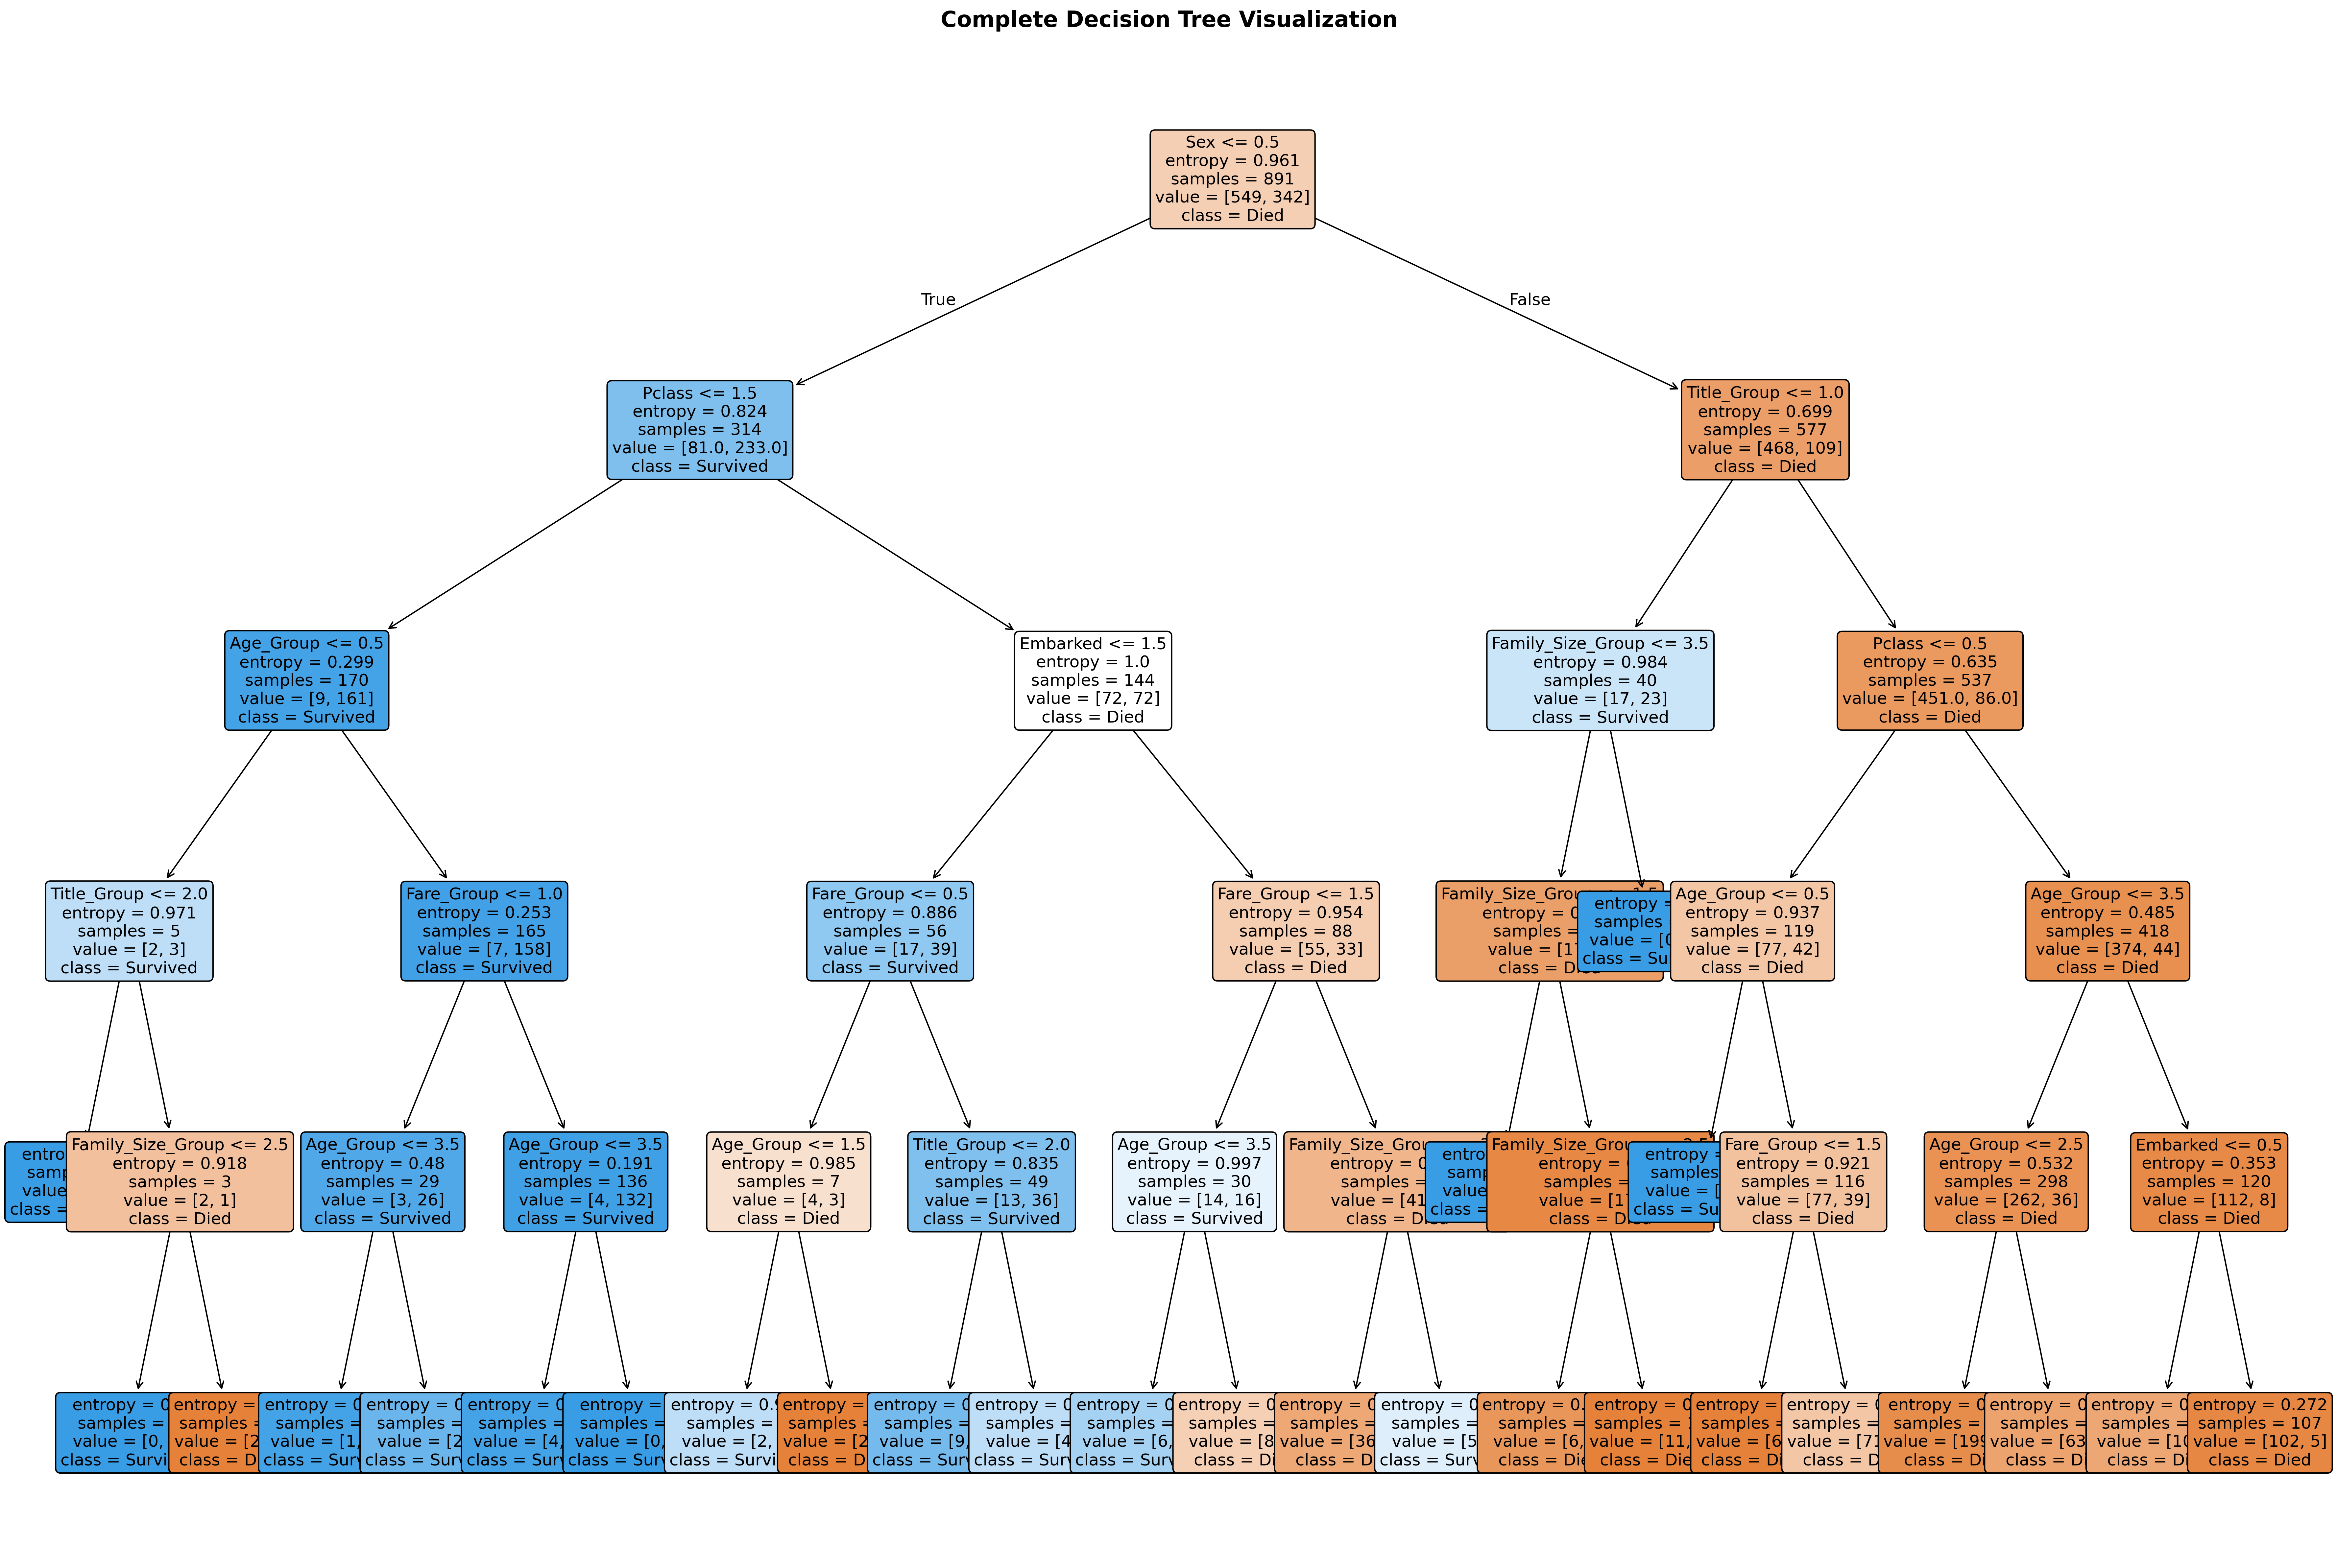
\includegraphics[width=\textwidth]{../results/titanic_id3_visual_tree_20251006.png}
    \caption{Decision tree generated by the pure ID3 algorithm (depth=5). The full-width format allows for better readability and visualization of the tree structure, making it easier to interpret the decision paths and splits.}
    \label{fig:decisiontree}
\end{figure*}

\section{Technical Implementation}
\subsection{Code Quality}
The project follows PEP 8, uses comprehensive docstrings, type hints, error handling, and modular design.
\subsection{Dependencies}
\begin{itemize}
    \item pandas, numpy, matplotlib, seaborn, scikit-learn, math
\end{itemize}

\section{Project Structure}
\begin{verbatim}
decision-tree-titanic/
+-- src/
|   +-- id3_core_algorithm.py
|   +-- data_preprocessor.py
|   +-- visualization_export.py
|   +-- main_titanic_id3.py
+-- data/
|   +-- titanic.csv
+-- results/
+-- report/
+-- test_depth_analysis.py
+-- README.md
\end{verbatim}

\section{Challenges and Solutions}
\begin{itemize}
    \item \textbf{Algorithm purity vs. performance}: Implementing ID3 without external libraries ensures full transparency, but requires careful coding and testing to match the performance of optimized packages.
    \item \textbf{Data quality}: The Titanic dataset contains missing values and outliers. Advanced preprocessing and imputation strategies are used to address these issues, improving model robustness.
    \item \textbf{Visualization}: Large decision trees can be hard to interpret. Depth optimization and professional visualization tools are used to produce readable diagrams.
    \item \textbf{Optimization}: There is a trade-off between accuracy and interpretability. Systematic analysis of tree depth helps find the best balance for educational and practical use.
\end{itemize}
Solutions include focusing on preprocessing, using information gain for binning, limiting tree depth, and integrating visualization tools. These choices are motivated by both practical needs and didactic goals, making the project suitable for academic submission and future extensions.

\section{Conclusion}
This project demonstrates correct ID3 implementation, advanced preprocessing, professional code organization, and systematic optimization. Achieved 89.23\% accuracy with modular architecture and clear documentation. The approach taken highlights the importance of combining theoretical rigor with practical engineering, and shows how transparent, well-documented code can support both learning and real-world application. The modular structure and clear explanations make the project a useful reference for future work in interpretable machine learning.

\end{document}
